\vspace{-2pt}\section{Experiments}
%%%%%%%%%%%%%%%%%%%%%%%%%%%%%%%%%%%%%%%%%%%%%%%%%%%%%%%%%%%%%%%%%%%%%%%%%%%
% Dataset description
%%%%%%%%%%%%%%%%%%%%%%%%%%%%%%%%%%%%%%%%%%%%%%%%%%%%%%%%%%%%%%%%%%%%%%%%%%%
\vspace{-2pt}\paragraph{The ADHD-200 Dataset.}
We used the publicly available ADHD-200 competition dataset \cite{ADHD200}, which contains rs-fMRI scans of subjects diagnosed as either typically developing (TD) or with ADHD. 
The dataset is collected across seven sites and consists of two parts: a training set and a validation test set (Brown site excluded from our study as the subject labels are not released).
Analyses were limited to participants with: 
(1)~MPRAGE anatomical images with consistent near-full brain coverage with successful registration; 
(2)~complete phenotypic information for main phenotypic variables (diagnosis, age, handedness); 
(3)~mean framewise displacement (FD) within two standard deviation (SD) of the sample mean;
(4)~full IQ within two SDs of the \mbox{ADHD-200} sample mean.
After applying these sample selection criteria, we analyzed resting state scans from $628$ individuals (TD${=}416$, ADHD${=}212$) in the training set and $106$ subjects (TD${=}65$, ADHD${=}41$) in the test set.
Functional images were reconstructed, slice-time corrected, motion corrected, and co-registered to the MNI space using SPM$8$.

%%%%%%%%%%%%%%%%%%%%%%%%%%%%%%%%%%%%%%%%%%%%%%%%%%%%%%%%%%%%%%%%%%%%%%%%%%%
% Experimental results
%%%%%%%%%%%%%%%%%%%%%%%%%%%%%%%%%%%%%%%%%%%%%%%%%%%%%%%%%%%%%%%%%%%%%%%%%%%
\vspace{-3pt}\paragraph{Experimental Results.}
To assess the validity of the proposed method, we compared the performance of various SVM-based classifiers using the ADHD-200 dataset, where resting-state FCs were produced using the parcellation scheme described in Sec.~\ref{sec:methods}.
For the intra-task penalty \RegA, we compared four different regularization schemes: Elastic-net (EN) \cite{Chen:2012b} with $\RegA(\w)=\frac{1}{2}\norm{\w}^2_2$, GN, FL, and TV.  
For the inter-task penalty \RegB, we compared three different approaches:
\begin{enumerate}[leftmargin=14pt]\vspace{-3pt}% http://tex.stackexchange.com/questions/91124/itemize-removing-natural-indent
	\item\textbf{Pooled} \ellone: a single classifier is trained on the entire ADHD-200 dataset ($\RegB(\wall)\,{=}\,\norm{\wall}_1$ with $\wall\,{\in}\,\Rp$ as $K\,{=}\,1$).
	\item \textbf{Single-task} \STL: equivalent to training separately across sites due to the separability of the penalty across sites ($\RegB(\wall)\,{=}\,\sum_{j=1}^p\norm{\w_j}_1)$.
	\item \textbf{Multitask} \MTL: \emph{jointly} train the classifiers by solving \eqref{eqn:erm2}.
\end{enumerate}\vspace{-3pt}
The regularization parameters $\{\lambda,\gamma\}$ are tuned by conducting a $5$-fold cross-validation (CV) on the training set over the following two-dimensional grid:
$\lambda,\gamma{\in}\{2^{-13},2^{-12},{\dots},2^{-3}\}$.
The final weight vector estimate is obtained by re-training the classifiers on the entire training set using the $\{\lambda,\gamma\}$ values that maximized the CV classification accuracy; 
for validation, we predicted the labels of the test set subjects using this weight vector.
All methods were solved using ADMM with the algorithm terminated when the condition 
\sloppy{$\norm{\wall^\text{new}-\wall^\text{old}}_2 \,{\leq}\,5{\cdot}10^{-3}{\times}\norm{\wall^\text{old}}_2$}
was met or the iteration count reached $400$.

\newcommand{\hsp}{\hspace{-1pt}}
%=========================================================================%
% introduce list of classification performance measures
%=========================================================================%
To evaluate the quality of the classifiers, we analyzed the following set of performance measures for both the \mbox{$5$-fold CV} and the validation test set results:
\begin{itemize}\vspace{-3pt}
	\item Classification accuracy (ACC) 
	\item Area under the ROC curve (AUC)
	\item Balanced score rate (BSR) $=$ (sensitivity+specificity)$/2$
	\item Stability score (Stab.) $=$ a measure of feature selection stability (see \cite{Baldassarre:2012, Rasmussen:2012})
	\item P-value (PVAL) computed from binomial test.
	\item Sparsity level (SP\%) $=100\cdot\frac{\abs{\text{\# non-zero features}}}{pK}$
\end{itemize}\vspace{-3pt}
The\hspace{-1pt} \emph{AUC} and \emph{BSR} are analyzed since \emph{ACC} by itself can be misleading when the dataset labels are imbalanced (ACC, \hsp AUC, and BSR are averaged across the tasks); the ROC curves are constructed by varying the threshold of the classifiers.
\emph{Stability score} is a measure introduced in \cite{Rasmussen:2012} which quantifies the stability of the features selected across the CV folds (see~\cite{Baldassarre:2012, Rasmussen:2012} for its precise definition).
Classifier performance on the test set was compared to random guessing via a binomial test based on a binomial distribution $B($p$,$n$)$ with p${=}0.5$ and n${=}109$ samples, with \emph{PVAL} evaluated via an one-sided binomial test~\cite{Heinzle:2012}; the alternative approach of permutation test was not pursued due to its severe computational \mbox{cost}.
Finally, \emph{sparsity level} is the fraction of features selected in the final model.

%-------------------------------------------------------------------------%
% Results Table & ROC
%-------------------------------------------------------------------------%
%!TEX root = paper.tex
\begin{figure}[t!]
		\captionof{table}{The classification results from the \mbox{$5$-fold CV} and the validation test-set.}\label{table:results}\vspace{-7pt}
		\centering
		\renewcommand{\FSIZE}[1]{\normalsize{#1}}
		\renewcommand{\HSPACE}{\hspace{-5.5pt}}
		\setlength{\tabcolsep}{2.7pt}
		\renewcommand{\arraystretch}{1.25} % space between rows
	\tfontsize{10.25}{
	\begin{tabular}{cc||cccc|ccccc}
		\specialrule{.8pt}{0em}{0em} 
		&& \multicolumn{4}{c|}{CV (628 subjects)}& \multicolumn{5}{c}{Test-set (106 subjects)}\\
		&& \FSIZE{ACC} & \FSIZE{AUC} & \FSIZE{BSR} & Stab. & \FSIZE{ACC}  & \FSIZE{AUC} & \FSIZE{BSR} & \FSIZE{PVAL} & SP\% \\
		 	\hline\hline
		  		     				% ACC(CV)  AUC(CV)   BSR(CV) 	(Stab)	ACC(TS)   AUC(TS)   BSR(TS)  		pval 	(NF)
		EN & \HSPACE\FSIZE{(\ellone)} 	& .689  	& .687	& .630	& .277	& .557 	& .617	& .476	& 	.143	& 2.54\%	\\
		GN & \HSPACE\FSIZE{(\ellone)} 	& .704  	& .708	& .631	& .253	& .594 	& .608	& .494	& 	.032	& 28.88\%	\\
		FL & \HSPACE\FSIZE{(\ellone)} 	& .688  	& .720	& .586	& .059	& .632 	& .592	& .530 	&	.004	& 64.85\%	\\
		TV & \HSPACE\FSIZE{(\ellone)} 	& .701  	& .715	& .620	& .005	& .623 	& .608	& .521 	&	.007	& 90.32\%	\\
			\hline 
		EN & \HSPACE\FSIZE{ (\STL)} 		& .709  	& .752	& .649	& .276	& .623 	& .609	& .530 	&	.007	& 0.28\%	\\
		GN & \HSPACE\FSIZE{ (\STL)} 		& .713  	& .750	& .652	& .165	& .642 	& .613	& .573 	&	.002	& 67.14\%	\\
		FL & \HSPACE\FSIZE{ (\STL)} 		& .715  	& .750	& .659	& .329	& .632 	& .634	& .547	&	.004	& 1.30\%	\\
		TV & \HSPACE\FSIZE{ (\STL)} 		& .718  	& .753	& .661	& .345	& .642 	& .654	& .550	&	.002	& 1.61\%	\\
			\hline 
		EN & \HSPACE\FSIZE{ (\MTL)} 		& .720  	& .754	& .657	& .217	& .651 	& .645	& .556	&	.001	& 0.25\%	\\
		GN & \HSPACE\FSIZE{ (\MTL)} 		& .720  	& .766	& .657	& .320 	& .642 	& .668	& .546	&	.002	& 1.03\%	\\
		FL & \HSPACE\FSIZE{ (\MTL)}		& .718  	& .766	& .653	& .315	& .642 	& .673	& .546	&	.002	& 0.79\%	\\
		TV & \HSPACE\FSIZE{ (\MTL)}		& .720 	& .766	& .658	& .316 	& .642 	& .672	& .546	&	.002	& 0.80\%	\\
		\specialrule{.8pt}{0em}{0em}
	\end{tabular}}\vspace{2pt}
	\label{table:reults,a}
	%=========================================================================%
	% figure
	%=========================================================================%
	\renewcommand{\imwidth}{130pt}
	\renewcommand{\imheight}{130pt}
		\renewcommand{\FSIZE}[1]{\tfontsize{9.75}{\textbf{#1}}}
		\centering
		\begin{tabular}{cc}
			\hspace{15pt}\FSIZE{CV (628 subjects)} &
			\hspace{15pt}\FSIZE{Test-set (128 subjects)} \\[-3pt]
			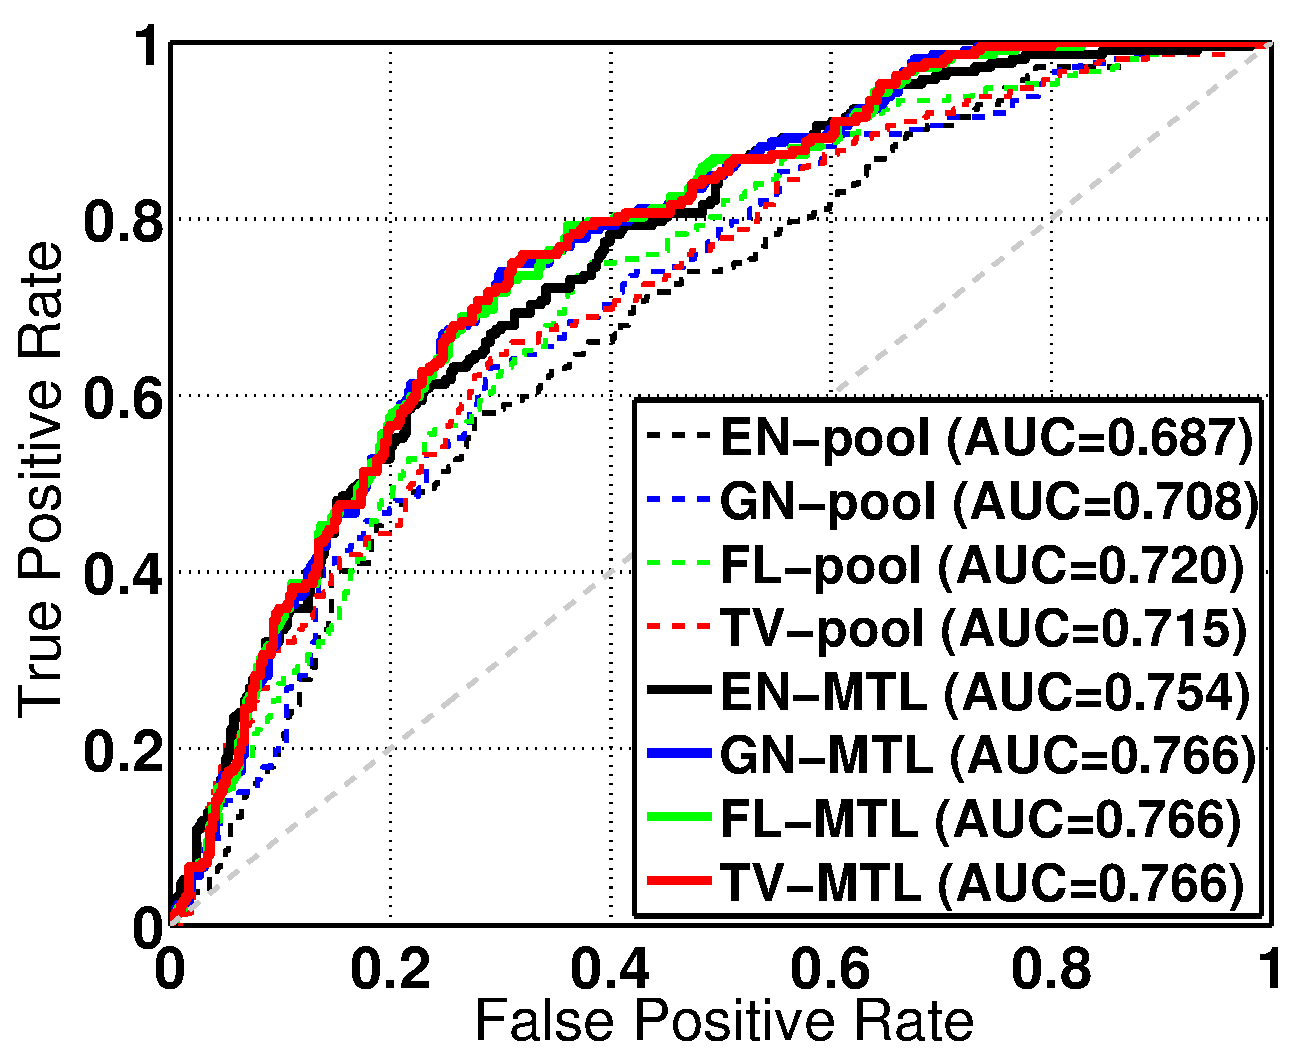
\includegraphics[width=\imwidth,height=\imheight]{\fig/roc_CV.pdf}&			
			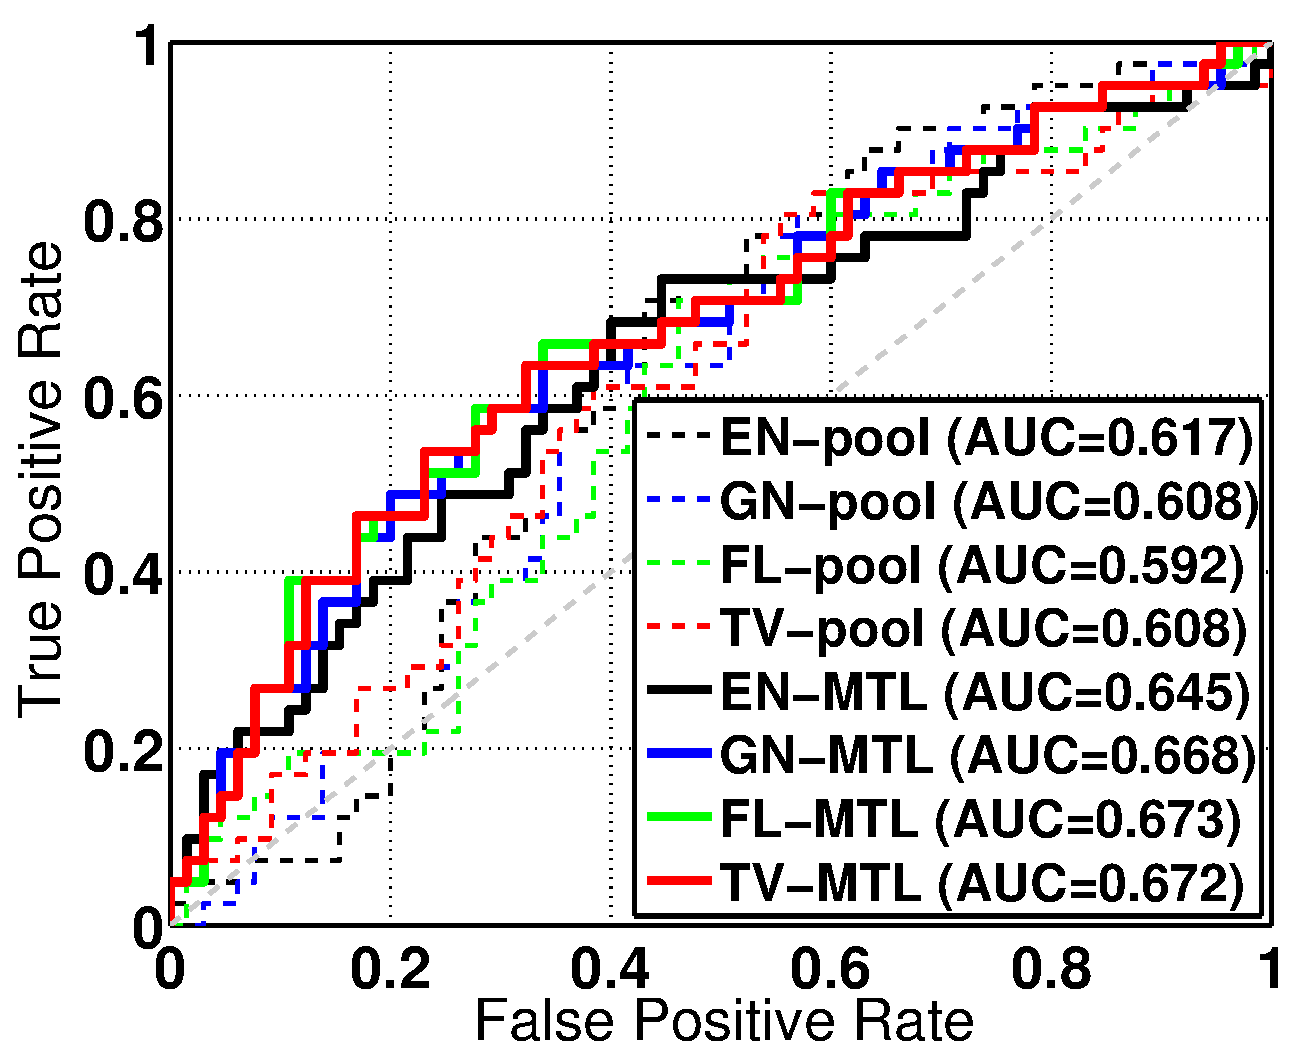
\includegraphics[width=\imwidth,height=\imheight]{\fig/roc_test.pdf}			
		\end{tabular}
		\label{fig:roc}
		\captionof{figure}{\tfontsize{9}{Table 1 classifiers' ROC (\STL-curves omitted to improve curve visibility).}}\vspace{-15pt}
\end{figure}


%=========================================================================%
% discussion on result on table1 and roc curve
%=========================================================================%
Table~\ref{table:results} presents the classification results from the \mbox{$5$-fold CV} and validation on the test-set, and Fig.~\ref{fig:roc} displays the corresponding ROC curves.
These results demonstrate that training a single classifier via the ``pooling'' approach yields the worst performance in terms of accuracy, AUC, and BSR, suggesting that blindly aggregating the datasets across different sites can be problematic for accurate disease classification. 
Comparison between the single-task and the multitask approaches shows that the \MTL-penalized approach  yields superior performance in terms of AUC, although no striking difference can be observed in terms of accuracy and BSR.

%=========================================================================%
% discussion on the results
%=========================================================================%
In addition to the performance gain with the \MTL-penalty, the set of weight vector estimates $\{\hat{\w}^k\}_{k=1}^K$ all share a common support of length $p$ with this multitask approach. 
This is invaluable for interpretation, as the selected features can be viewed as edges that are informative across all sites.
For visualization, we grouped the indices of this support according to the network parcellation scheme proposed by Yeo \etal in~\cite{Yeo:2011}, and reshaped them into a $347{\times}347$ symmetric matrix with zeroes on the diagonal. 
The resulting support matrices for the EN+\MTL and the FL+\MTL-penalized SVM are presented in Fig.\hspace{2.5pt}\ref{fig:weight} (results for GN+\MTL and TV+\MTL were very similar to FL+\MTL).
An interesting observation here is that the support structure from the FL+\MTL-penalized SVM shows concentrated connectivity patterns in the intra-frontoparietal \mbox{(6-6)} and the intra-default network (7-7) regions; Fig.~\ref{fig:weight} provides a brain space representation of these connections (figures generated using BrainNet Viewer, \url{www.nitrc.org/projects/bnv/}).
These network regions are frequently reported to exhibit disrupted connectivity patterns in resting state studies of ADHD~\cite{Castellanos:2012}, although the accuracies obtained from our classifiers are not at the level where the selected features can be interpreted as reliable ADHD biosignatures. 

\vspace{-.75pt}
Finally, we note that most of the accuracies reported on the validation test-set in Table~\ref{table:results} exceeded the highest result from the actual  ADHD-200 competition (which was $61.54\%$~\cite{ADHD200}).
However, there are two major caveats:
(1) the results in this work cannot be directly compared with the official competition results due to the subject screening procedure we applied on the test set (the criteria such as the FD-based one is important for avoiding  confounds from excessive head motion), and
(2) the participants in the actual competition were required to predict the labels of $26$ subjects from the Brown site, despite the fact that no training data were provided from this site, making it harder to predict the labels for these subjects.
The second caveat also implies that most MTL methods, including the \MTL-penalty employed in this work, cannot be applied since there are no means to train a weight vector for a task whose data are not provided.
An alternative approach such as \emph{transfer learning}~\cite{Pan:2010} may be considered for this.

%-------------------------------------------------------------------------%
% Results: Brain-net viewer
%-------------------------------------------------------------------------%
\begin{figure}[t!]
	%=====================================================================%
	% yeo table
	%=====================================================================%
	\newcommand{\yeofont}[1]{\small{#1}}
	\setlength{\tabcolsep}{5.5pt}
	\renewcommand{\arraystretch}{0.97} % space between rows
	\captionof{table}{Network parcellation scheme of the brain proposed by Yeo \etal in \cite{Yeo:2011}.}
	\vspace{-6pt}\begin{tabular}{llll}
		\hline
		\multicolumn{4}{c}{\textbf{\small{Network membership Table ($\times$ is ``unlabeled'')}}}  \\ 
		\hline\hline
		 \yeofont{1. Visual}	& \yeofont{2. Somatomotor}	& \yeofont{3. Dorsal Attention} & \yeofont{4. Ventral Attention}  \\[-2pt]
		 \yeofont{5. Limbic} 	& \yeofont{\doblue{6. Frontoparietal}} & \yeofont{\dored{7. Default}} 	& \yeofont{8. Striatum} \\[-2pt]
		 \yeofont{9. Amygdala} & \yeofont{10. Hippocampus} & \yeofont{11. Thalamus}	& \yeofont{12. Cerebellum} \\[-1.5pt]
		\hline \\[-4pt]
	\end{tabular}
	%=====================================================================%
	% figures
	%=====================================================================%
	\renewcommand{\imwidth}{120pt}
	\renewcommand{\imheight}{61.0pt}
	\renewcommand{\arraystretch}{1.00} % space between rows
	\setlength{\tabcolsep}{3.85pt}	
	\renewcommand{\VSPACE}{\vspace{-100pt}}
	\begin{tabular}{cc}
		%=================================================================%
		% elastic net
		%=================================================================%
		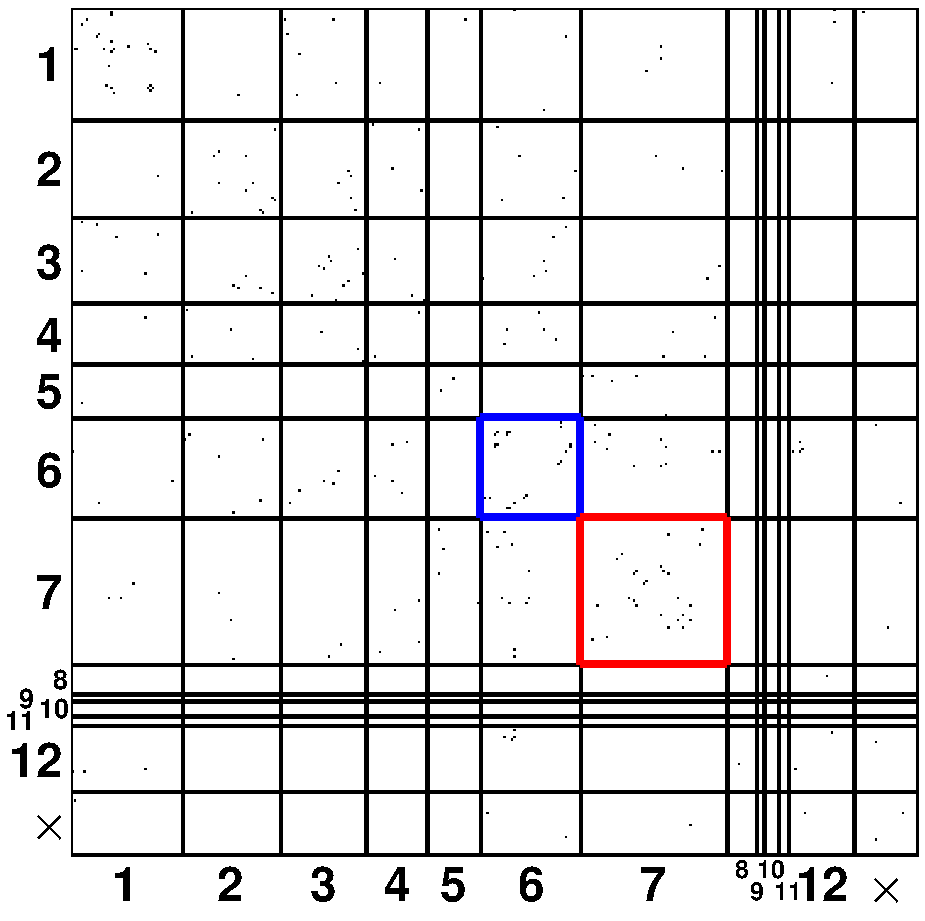
\includegraphics[width=\imwidth]{weight_enet.pdf} \hspace{1pt}
		&
		\begin{tabular}{ccc}
		\vspace{-135pt} \\
			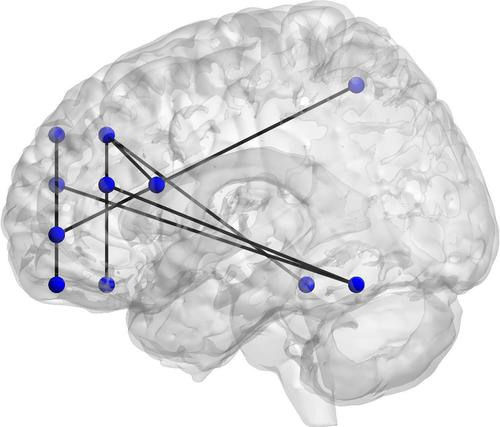
\includegraphics[height=\imheight]{6-6enet_lateral.jpg} & 
			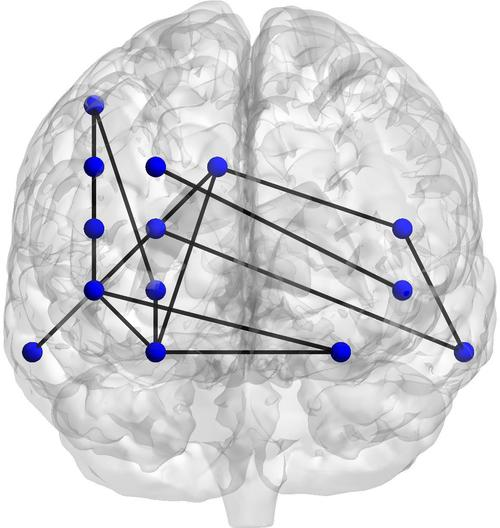
\includegraphics[height=\imheight]{6-6enet_anterior.jpg} & 
			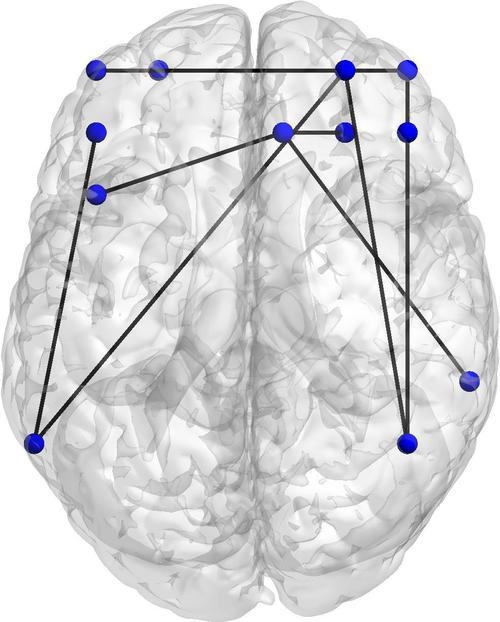
\includegraphics[height=\imheight]{6-6enet_superior.jpg} \\[-1.5pt]
			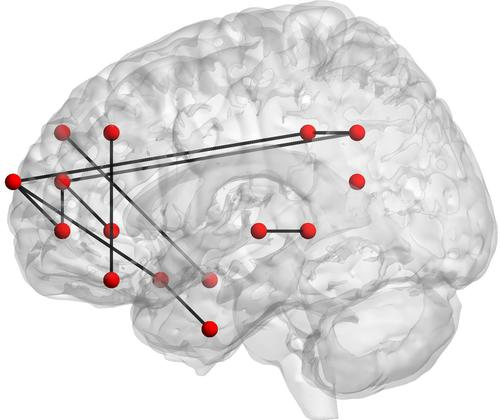
\includegraphics[height=\imheight]{7-7enet_lateral.jpg} & 
			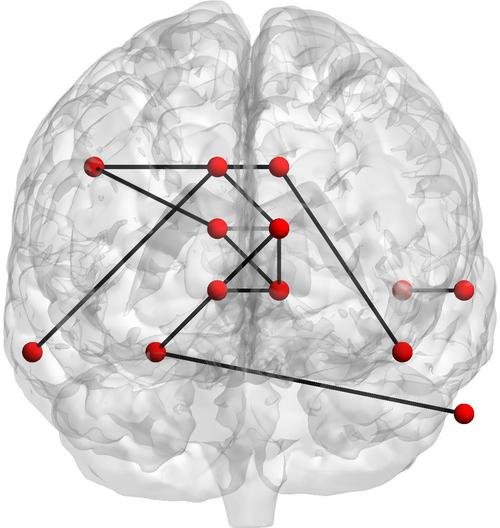
\includegraphics[height=\imheight]{7-7enet_anterior.jpg} & 
			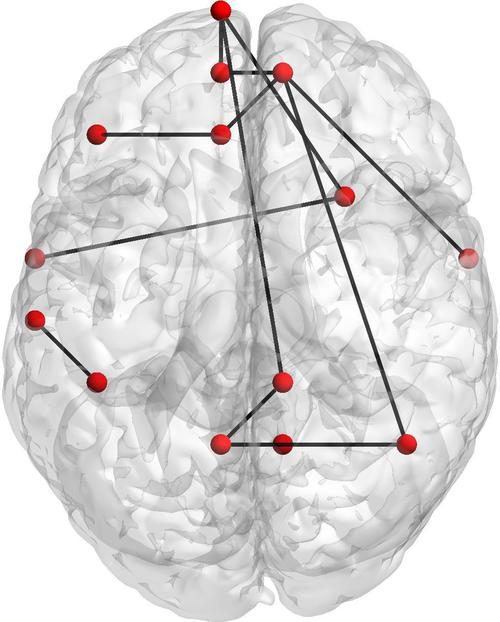
\includegraphics[height=\imheight]{7-7enet_superior.jpg} \\[-3.5pt]
		\end{tabular} \\[-0pt]
		\multicolumn{2}{c}{\small{\textbf{(a)} Multitask Elastic-net SVM result}}\\[12pt]
		%=================================================================%
		% fused lasso
		%=================================================================%
		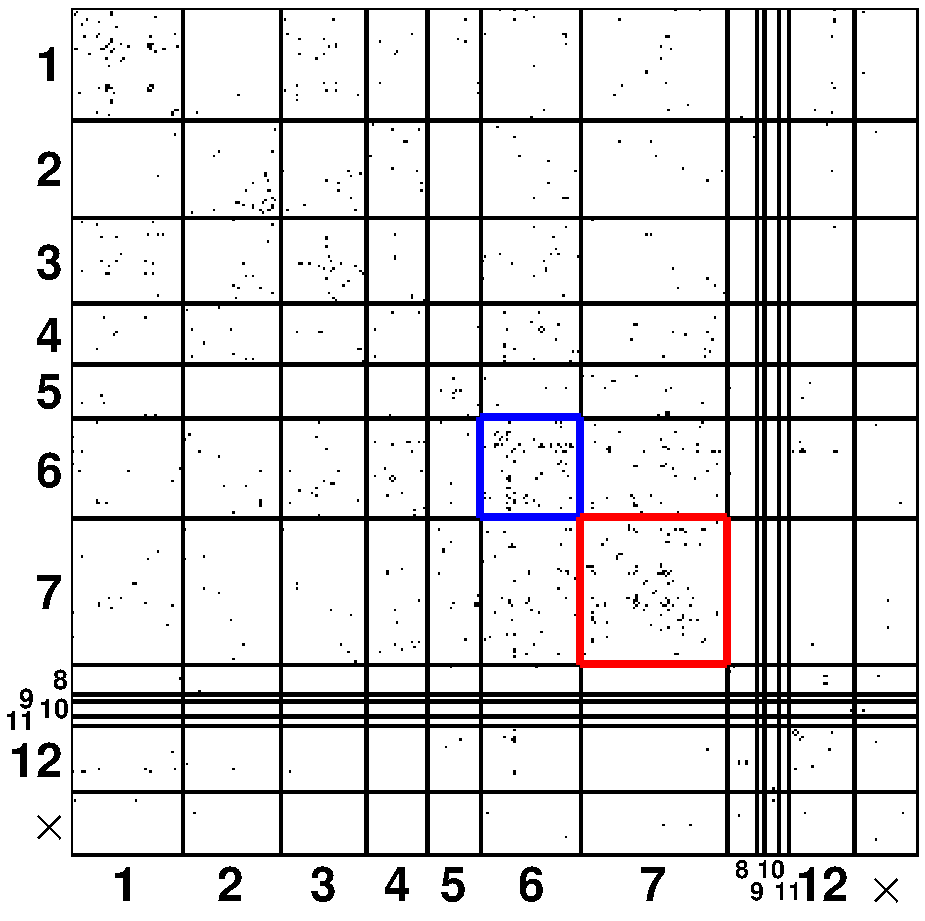
\includegraphics[width=\imwidth]{weight_flas.pdf} \hspace{1pt}
		&
		\begin{tabular}{ccc}
		\vspace{-135pt} \\
			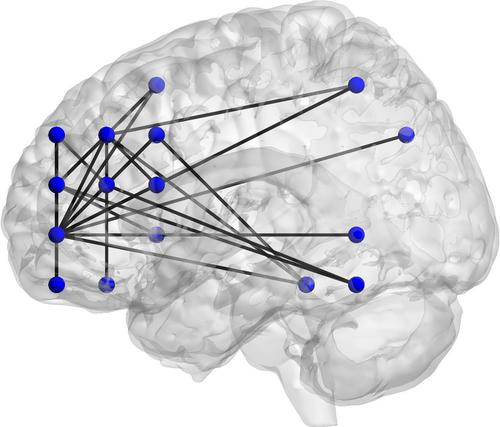
\includegraphics[height=\imheight]{6-6flas_lateral.jpg} & 
			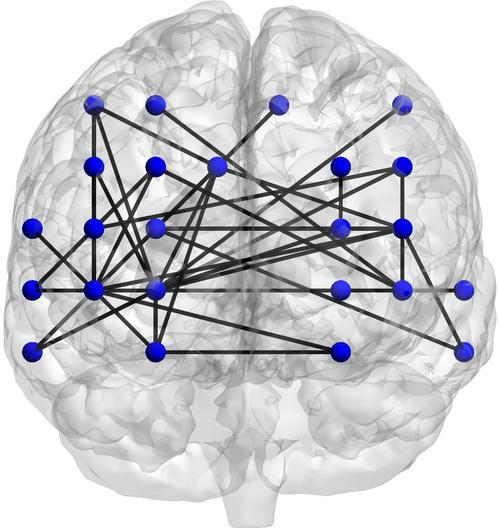
\includegraphics[height=\imheight]{6-6flas_anterior.jpg} & 
			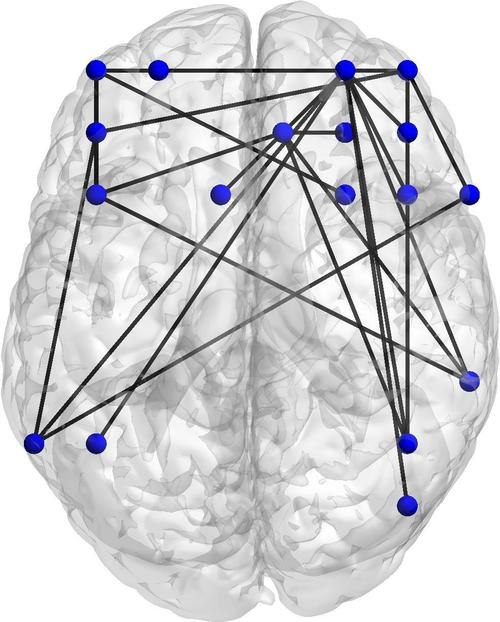
\includegraphics[height=\imheight]{6-6flas_superior.jpg} \\[-1.5pt]
			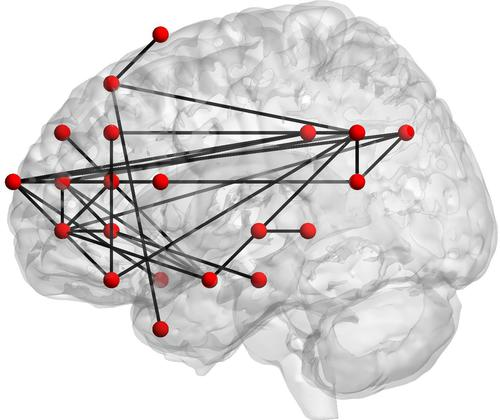
\includegraphics[height=\imheight]{7-7flas_lateral.jpg} & 
			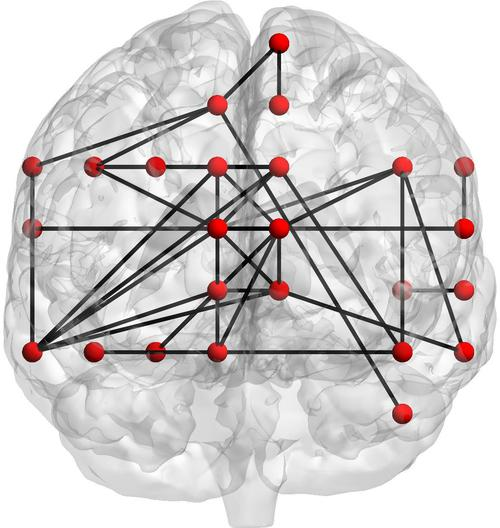
\includegraphics[height=\imheight]{7-7flas_anterior.jpg} & 
			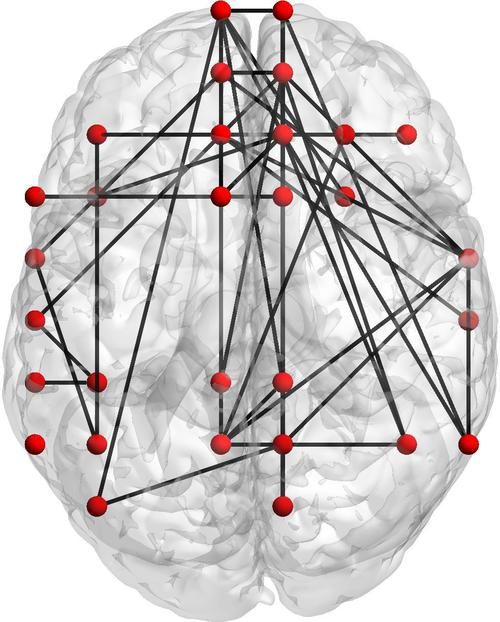
\includegraphics[height=\imheight]{7-7flas_superior.jpg} \\[-3.5pt]
		\end{tabular}  \\
		\multicolumn{2}{c}{\small{\textbf{(b)} Multitask Fused Lasso SVM result}}\\[3pt]
	\end{tabular} 
	\captionof{figure}{
	Weight vectors estimated from the EN+\MTL and FL+\MTL-penalized SVM.
	\textbf{Left:} support matrices of the selected features (rows/cols grouped by network membership).
	\textbf{Right:} brain space representation of the selected edges in the intra-frontoparietal (\mbox{6-6}: blue) and the intra-default network (7-7: red).
	}
	\label{fig:weight}
	\vspace{-14pt}
\end{figure}



